\documentclass{article}
\usepackage{graphicx}
\usepackage{hyperref}

\usepackage{Sweave}
\begin{document}
\Sconcordance{concordance:RCircos.tex:RCircos.Rnw:%
1 4 1 1 0 38 1 1 3 5 0 1 2 4 1 1 2 1 0 1 1 12 0 1 2 3 1 1 2 1 0 1 1 19 %
0 1 2 4 1 1 2 1 0 1 1 12 0 1 2 79 1 1 4 44 0 2 1 19 0 1 2 5 1 1 4 3 0 1 %
1 1 2 1 0 1 3 4 0 1 2 11 1 1 5 4 0 1 1 1 2 1 0 1 1 3 0 1 2 11 1 1 5 7 0 %
1 2 9 1 1 5 4 0 1 2 1 0 1 3 1 0 1 2 1 0 2 1 2 2 1 0 2 2 4 0 1 2 5 1 1 4 %
3 0 1 2 1 0 1 2 2 1 1 2 4 0 1 2 1 4 3 0 1 1 1 2 2 1 1 4 5 0 1 2 1 4 3 0 %
1 2 1 0 1 2 2 1 1 4 5 0 1 2 1 4 3 0 1 2 1 0 1 2 2 1 1 3 5 0 1 2 1 4 3 0 %
1 2 1 0 1 2 1 1 1 2 4 0 1 2 8 1 1 4 3 0 1 1 1 3 2 0 1 2 3 0 1 2 9 1 1 2 %
1 0 1 4 5 0 1 2 1 4 6 0 1 2 1 1 1 2 20 0 1 2 5 1}


\title{Using the RCircos Package}
\author{Hongen Zhang, Ph.D.\\
Genetics Branch, Center for Cancer Research,\\
National Cancer Institute, NIH}
\date{February 12, 2013}
\maketitle

\tableofcontents

\section{Introduction}

The RCircos package provides a set of graphic functions which implement basic Circos 2D track plot \cite{Krzywinski} for visualizing similarities and differences of genome structure and positional relationships between genomic intervals. The package is implemented with R graphics package that comes with R base installation and aimed to reduce the complexity of usage and increase the flexibility in integrating into other R pipelines of geneomic data processing. Curently, following graphic functions are provided: 

\begin{itemize}
\item
Chromosome ideogram plots for human, mouse, and rat
\item
Data plots include:
\begin{itemize}
  \item heatmap
  \item histogram 
  \item lines 
  \item scatterplot 
  \item tiles
\end{itemize}
\item
Plot items for further decoration include:
\begin{itemize}
  \item connectors
  \item links
  \item text (gene) labels
\end{itemize}
\end{itemize}

After successful installation of RCircos, one needs to load the library to get started using it.

\begin{Schunk}
\begin{Sinput}
> # load the library
> library(RCircos)
\end{Sinput}
\end{Schunk}

\section{Input Data Format}

RCircos takes the input data in the form of a data frame that could be an object returned from read.table() or generated with other pipelines in the current R session. The first three columns of the data frame, except for input to the link plot,  must be genomic position information in the order of chromosome names, chromosome start, and chromosome end positions. 

\begin{Schunk}
\begin{Sinput}
> data(RCircos.Histogram.Data)
> head(RCircos.Histogram.Data)
\end{Sinput}
\begin{Soutput}
  Chromosome chromStart chromEnd     Data
1       chr1   45000000 49999999 0.070859
2       chr1   55000000 59999999 0.300460
3       chr1   60000000 64999999 0.125421
4       chr1   70000000 74999999 0.158156
5       chr1   75000000 79999999 0.163540
6       chr1   80000000 84999999 0.342921
\end{Soutput}
\end{Schunk}


For gene labels and heatmap plots, the gene/probe names must be provided in the fourth column. For other plots, this column could be optional. 

\begin{Schunk}
\begin{Sinput}
> data(RCircos.Heatmap.Data)
> head(RCircos.Heatmap.Data)
\end{Sinput}
\begin{Soutput}
  Chromosome chromStart chromEnd GeneName  X786.O     A498 A549.ATCC    ACHN
1       chr1     934341   935552     HES4 6.75781  7.38773   6.47890 6.05517
2       chr1     948846   949919    ISG15 7.56297 10.49590   5.89893 7.58095
3       chr1    1138887  1142089 TNFRSF18 4.69775  4.55593   4.38970 4.50064
4       chr1    1270657  1284492     DVL1 7.76886  7.52194   6.87125 7.03517
5       chr1    1288070  1293915    MXRA8 4.49805  4.72032   4.62207 4.58575
6       chr1    1592938  1624243 SLC35E2B 8.73104  8.10229   8.36599 9.04116
    BT.549  CAKI.1
1  8.85062 7.00307
2 12.08470 7.81459
3  4.47525 4.47721
4  7.65386 7.69733
5  5.66389 4.93499
6  9.24175 9.89727
\end{Soutput}
\end{Schunk}


Different from other plot data, the input data for link line plot has only paired genomic position information for each row in the order of chromosome name A, chromStart A, chromEnd A, chromosome name B, chromStart B, and chromEnd B.


\begin{Schunk}
\begin{Sinput}
> data(RCircos.Link.Data)
> head(RCircos.Link.Data)
\end{Sinput}
\begin{Soutput}
  Chromosome chromStart  chromEnd Chromosome.1 chromStart.1 chromEnd.1
1       chr1    8284703   8285399         chr1      8285752    8286389
2       chr1   85980143  85980624         chr7    123161313  123161687
3       chr1  118069850 118070319         chr1    118070329  118070689
4       chr1  167077258 167077658         chr1    169764630  169764965
5       chr1  171671272 171671550         chr1    179790879  179791292
6       chr1  174333479 174333875         chr6    101861516  101861840
\end{Soutput}
\end{Schunk}


Note: RCircos will convert the input data to Circos plot data but it dose not provide functionality for general data processing. If the data frame does not have genomic position information, you have to add the information to the data frame before passing it to RCircos functions. Sample datasets are included in the package for demo purpose and they could be easily explored with data() mathod. 



\section{Plot Track Layout}

RCircos follows the same algorithm of Circos plot and arranges data plots in tracks. A track could be placed either inside or outside of chromosome ideogram and the detailed position fo a track could be easily manipulated by changing  of the track width and track numbers.


The figure below shows a human chromosome ideogram plus three empty tracks arranged in both inside and outside of chromosome ideogram.

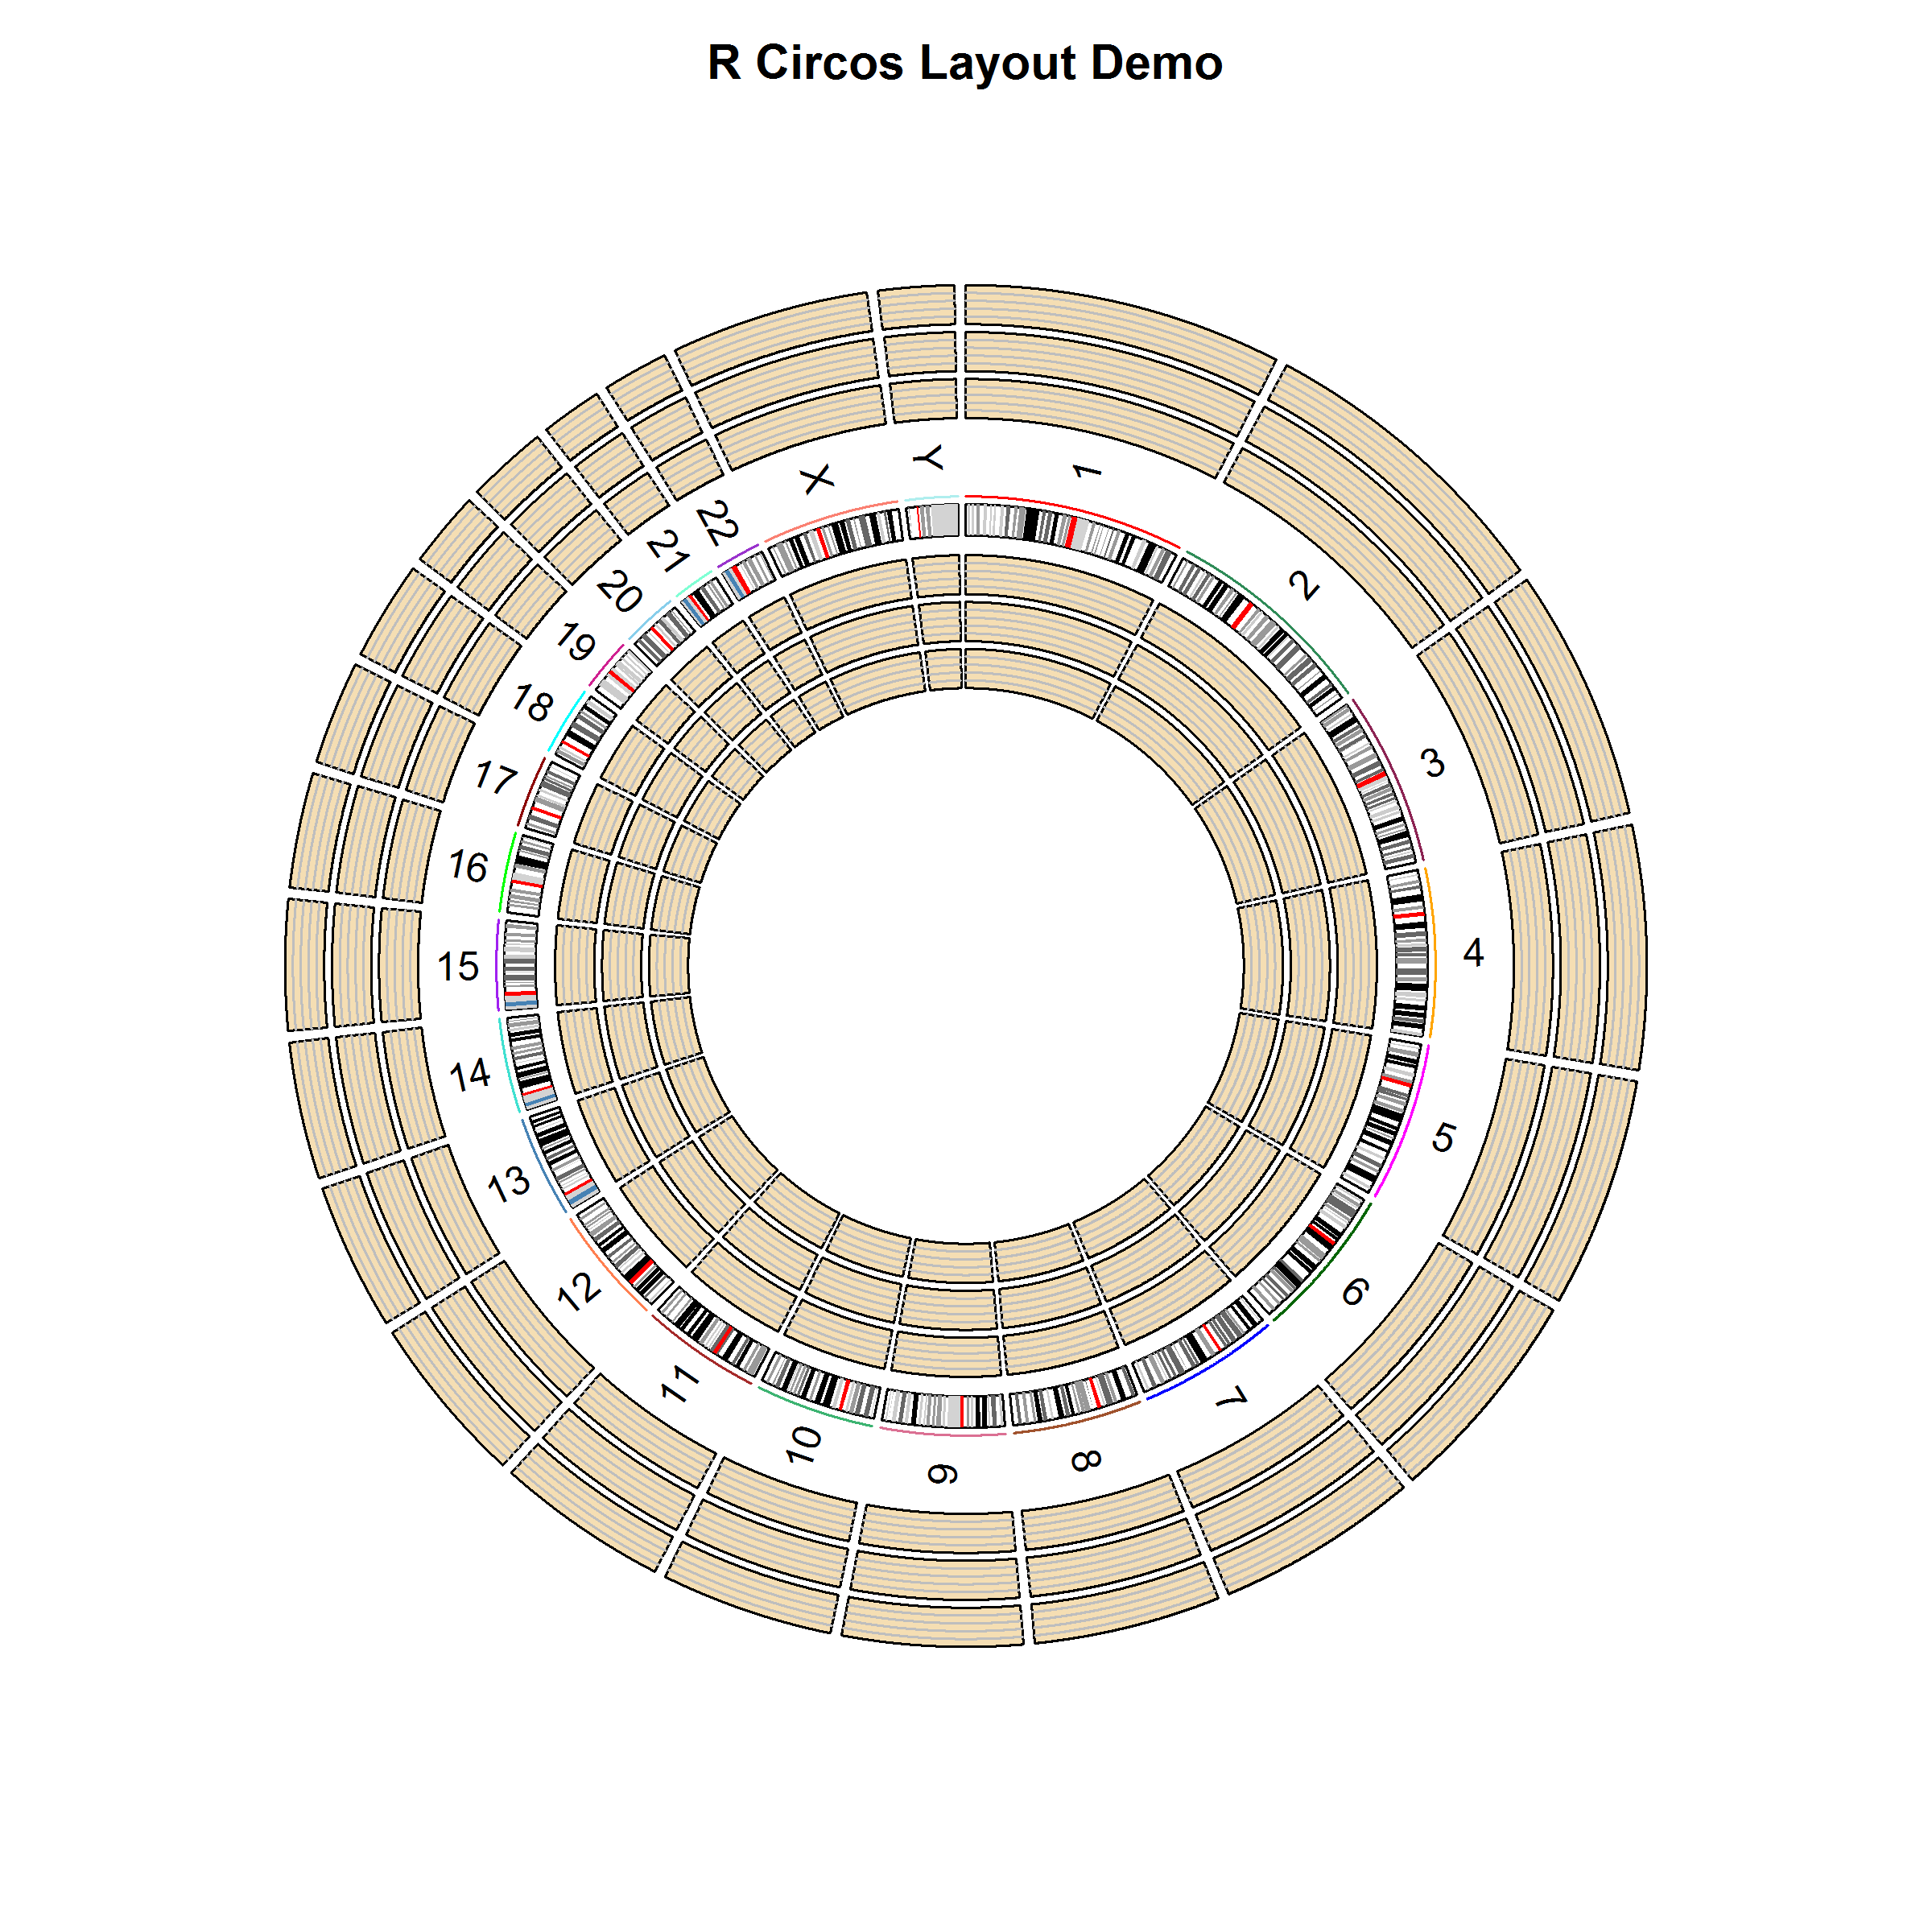
\includegraphics[width=1\textwidth]{RCircosLayoutDemo.png}


\section{Getting Started: Preliminary Steps for RCircos}

\subsection{Initialize Plot Parameters}

The first step of making RCircos plot is to initialize plot parameters. Following are plot parameters and their default values:

\begin{description}
\item[radiu.len] 
The radius of a circular line which serves as baseline for
calculation of plot items, default: 1
\item[chr.ideog.pos]
Radius of chromosome ideogram position, default: 1.1
\item[highlight.pos]
Radius of chromosome ideogram highlights, default: 1.2
\item[chr.name.po]
Radius of chromosome name position, default: 1.3
\item[plot.radius]
Radius of plot area,default: 1.5
\item[track.in.start]
Radius of start position of the first track inside of chromosome idogram, default: 1.05
\item[track.out.start]
Radius of start position of the first track outside of chromosome idogram, default: 1.4

\medskip  

\item[chrom.width]
Width of chromosomes of the ideogram, default: 0.08
\item[track.padding]
Width of padding between two plot tracks, default: 0.02
\item[track.height]
Height of data plot track, default: 0.1
\item[  ]
(Note: Parameters above are all relative to the radius.len).

\smallskip  
    
\item[base.per.unit]
Number of base pairs a chromosome unit (a plot point) will cover, default: 3000
\item[chrom.paddings]
Width of padding between two chromosomes in chromosome unit, default: 3000

\medskip  
  
\item[hist.width]
Width of histogram column in chromosome unit, default: 1000
\item[heatmap.width]
Width of heatmap cells in chromosome unit, default: 100
\item[max.layers]
Maximum number of layers for tile plot, default: 5

\smallskip  
  
\item[highlight.width]
Line type (same as lty in R graphics package) for chromosome highlight, default: 1
\item[text.size]
Character size (same as cex in R graphics package) for text plot, default: 0.4
\item[point.type]
Point type (same as pch in R graphics package) for scatter plot, default: "."
\item[point.size]
Point size (same as cex in R graphics package) for scatter plot, default: 1
\end{description}

Current values of plot parameters could be checked at anytime by calling RCircos.List.Parameters(). While the parameters could be modified anytime for a new plot during the R session, several parameters such as positions of chromosome ideogram, chromosome highlighs, chromosome names, first track inside and outside chromosome ideogram, and plot area are derived from radius.len so must be reset with the function of RCircos.Reset.Ideogram.Position(radiu.len), if radius.len is changed.

\begin{Schunk}
\begin{Sinput}
> #	Initialize plot parameters and reset circos radius
> #	**************************************************
> circpar <- RCircos.Initialize.Parameters();
\end{Sinput}
\begin{Soutput}
Parameters initialized.

radius.len:	 1 
chr.ideog.pos:	 1.1 
highlight.pos:	 1.2 
chr.name.pos:	 1.3 
plot.radius:	 1.5 
track.in.start:	 1.05 
track.out.start: 1.4 
chrom.width:	 0.08 
track.padding:	 0.02 
track.height:	 0.1 

base.per.unit:	 3000 

chrom.paddings:	 3000 
highlight.width:	 1 
hist.width:	 1000 
text.size:	 0.4 
heatmap.width:	 100 

point.type:	 . 
point.size:	 1 
max.layers:	 5 

Note: Following parameters are derived form radius.len:

chr.ideog.pos
highlight.pos
chr.name.pos
track.in.start
track.out.start
plot.radius

Reset them with RCircos.Reset.Ideogram.Position(radius.len)
when radius.len is changed. All other parameters could be 
modified from command line.
\end{Soutput}
\begin{Sinput}
> radius.len <- 2.5;
> circpar <- RCircos.Reset.Ideogram.Position(circpar, radius.len);
\end{Sinput}
\begin{Soutput}
Chromosome ideogram position reset:

radius.len 2.5 
chr.ideog.pos 2.6 
highlight.pos 2.7 
chr.name.pos 2.8 

track.in.start 2.55 
track.out.start 2.9 

plot.radius 3 

Increase value of plot.radius if there are plot tracks
outside of chromosome ideogram
\end{Soutput}
\end{Schunk}


\subsection{Get Base Plot Positions Based on A Chromosome Ideogram}

RCircos generates Circos images with points, lines, polygon, and text functions provided by R graphich package. To plot chromosome ideogram and data tracks in circular layout, RCircos needs a set of point positions that forms a circular line to serve as the baseline for x- and y-coordinates calculation of any plot items. The baseline positions has a defaul radius of 1 and number of total points are genome length in base pairs devided by chromosome units length (base.per.unit, base pairs a point will cover).  To get the baseline positions, run following code:

\begin{Schunk}
\begin{Sinput}
> #	Get cytoband data and calculate base positions
> #	**********************************************
> data(UCSC.HG19.Human.CytoBandIdeogram);
> cyto.info <- UCSC.HG19.Human.CytoBandIdeogram;
> cyto.band <- RCircos.Cytoband.Data(cyto.info, 
+ 			chr.exclude=NULL, circpar);
> circle.positions <- RCircos.Base.Plot.Positions(cyto.band, 
+ 			circpar);
\end{Sinput}
\end{Schunk}

As show above, the baseline positions are calculated based on cyto.band information (species specific). Currently, RCircos provides chromosome ideogram data for human, mouse, and rat queried from UCSC genome browser \\ 
(http://genome.ucsc.edu). Other species should work if ideogram data is provided with a tab-delimted text file with same column and column headers. In that case, use read.table() to get the cyto.info object.


\section{Making a Plot with RCircos}
Plotting with RCircos is a stepwise process.  First, an initialization step is needed.  Then, tracks and other aspects of the plot are added sequentially.  The result is available after the plot has been entirely constructed.  The next subsections walk through the process in detail.

\subsection{Initialize Graphic Device}

RCircos provides a set of graphic plot functions but does not handle graphic devices. To make RCircos plots, a graphic device has to be opened first. Currently, RCircos works with files supported by R graphics package such as tiff, png, pdf images as well as GUI windows.  For example, to make a pdf file with Circos plot image:

\begin{Schunk}
\begin{Sinput}
> #pdf.file <- "RCircosDemoHumanGenome.pdf";
> #pdf(file=pdf.file, height=8, width=8);
> 
> par(mai=c(0.25, 0.25, 0.25, 0.25));
> plot.new();
> plot.window(c(-1*circpar$plot.radius, circpar$plot.radius), 
+ 	c(-1*circpar$plot.radius, circpar$plot.radius+0.25));
> title("RCircos 2D Track Plot with Human Genome");
\end{Sinput}
\end{Schunk}


Note: Please make sure there is enough space for data track plotting by checking plot.radius, track.height and track.padding. By defaul, radius.len is 1 and track.height plus track.padding is 0.12. These default settings allow only a few tracks to be plotted inside of chromosome ideogram. For more data track plots, increase the radius.len and start over.


Note: After everything is done, the graphic device need to be closed with dev.off().


\subsection{Chromosome Ideogram}

After initializing plot parameters and acquiring cytoband data and base plot positions, a common first step is to draw chromosome ideograms and label chromosomes with names and highlights. Simply call and pass necessary arguments to RCircos.Chromosome.Ideogram() to add the ideogram to the current plot. 

\begin{Schunk}
\begin{Sinput}
> #	Draw chromosome ideogram
> #	*********************************
> RCircos.Chromosome.Ideogram(cyto.band, circle.positions, 
+ 			circpar);
\end{Sinput}
\end{Schunk}


\subsection{Gene Labels and connectors on RCircos Plot}

Label gene names with RCircos reqires one more step than other plots above, i.e., check and reset, if necessary, gene label positions in order to avoid overlap of neighbour gene names. Due to the resolution issues, only limited number of gene names can be labeled. For best visualization, cex should be no less than 0.4 when draw gene labels. When cex is set to 0.4, width of character will be 5000 chromosome units. If the gene name list supplied is too long, it will be truncted to fit the chromosome length. Also the long gene name will span more than one track so one or more tracks may need be skipped when calculate position for next track.

Connectors are used to mark a genomic positions with their names or variant status. Each connector consists two vertical lines and one connection line between two vertical lines. Each end of the connector points to the genomic position of one of two neighbour tracks (e.g, the chromosome ideogram and gene names). The connector data derived from input data should contains two plot positions to present the two ends of connector. When one end points to chromosome ideogram and another end points to the data track, connector data could be converted from input data by call RCircos.Get.Label.Locations(). If both ends are data tracks, process the input data for the track close to chromosome ideogram with function of RCircos.Get.Plot.Data() and convert the input data for the other track with function of RCircos.Get.Label.Locations(), then combine the last column of the first output and the last column of second output as connector data.

The following code uses gene data as plot data for RCircos.Connector() function to draw connectors between chromosome ideogram and gene names.

\begin{Schunk}
\begin{Sinput}
> #	Plot connectors in first track and gene
> #	names in the second track. 
> #	***************************************
> data(RCircos.Gene.Label.Data);
> label.data <- RCircos.Get.Plot.Data(RCircos.Gene.Label.Data, 
+ 			cyto.band);
> gene.data <- RCircos.Get.Label.Locations(cyto.band, 
+ 			label.data, label.type="text", circpar);
> conn.data <- data.frame(gene.data$Location, 
+ 			gene.data$Label.Position);
> name.col <- 4;
> direction <- "in";
> track.num <- 1;
> RCircos.Connector(cyto.band, circle.positions, 
+ 	conn.data, track.num, direction, circpar);
> track.num <- 2;
> RCircos.Gene.Label(circle.positions, gene.data, 
+ 	name.col, track.num, direction,  circpar);
\end{Sinput}
\end{Schunk}


\subsection{Heatmap, Histogram, Line, Scatter, and Tile Plot}

Heatmap, histogram, line, scatter, and tile plot with RCircos require that the first three columns of input data are genomic position information in the order of chromosome name, start, and end position. Before plot data track, the input data needs to be transformed to plot data. RCircos.Get.Plot.Data(input.Data, cyto.band) will perform this transformation. After the plot data is done, call relative function to plot the data on one or more selected track.

\begin{Schunk}
\begin{Sinput}
> #	Heatmap plot. 
> #	**************************************************
> data(RCircos.Heatmap.Data);
> expr.data <- RCircos.Get.Plot.Data(RCircos.Heatmap.Data, 
+ 				cyto.band);
> track.num <- 5;     # put in the fifth track
> direction <- "in";  # track is inside of chromosome ideogram
> data.col <- 6;      # column of data frame with plot data
> RCircos.Heatmap(cyto.band, circle.positions, expr.data, 
+ 			data.col, track.num, direction, circpar);
\end{Sinput}
\end{Schunk}

\begin{Schunk}
\begin{Sinput}
> #	Scatterplot with DNA copy number variation data
> #	**********************************************
> data(RCircos.Scatter.Data);
> scatter.data <- RCircos.Get.Plot.Data(RCircos.Scatter.Data, 				cyto.band);
> track.num <- 6; 
> direction <- "in";
> data.col <- ncol(scatter.data)-1;
> RCircos.ScatterPlot(cyto.band, circle.positions, 
+ 		scatter.data, data.col, track.num,  
+ 		direction, by.fold=1, circpar);
\end{Sinput}
\end{Schunk}

\begin{Schunk}
\begin{Sinput}
> #	Line plot with DNA copy number variation data
> #	**********************************************
> data(RCircos.Line.Data);
> line.data <- RCircos.Get.Plot.Data(RCircos.Line.Data, 
+ 		cyto.band);
> track.num <- 7;
> direction <- "in";
> data.col <- ncol(line.data)-1;
> RCircos.Line.Plot(cyto.band, circle.positions, 
+ 			line.data, data.col, 
+ 			track.num, direction, circpar);
\end{Sinput}
\end{Schunk}

\begin{Schunk}
\begin{Sinput}
> #	Draw Histogram
> #	**********************************************
> data(RCircos.Histogram.Data);
> hist.data <- RCircos.Get.Plot.Data(RCircos.Histogram.Data, 
+ 			cyto.band);
> track.num <- 8; 
> direction <- "in";
> data.col <- 4;
> RCircos.Histogram(cyto.band, circle.positions, 
+ 			hist.data, data.col, 
+ 			track.num, direction, circpar);
\end{Sinput}
\end{Schunk}

\begin{Schunk}
\begin{Sinput}
> #	Draw Tile plot. 
> #	**********************************************
> data(RCircos.Tile.Data);
> tile.data <- RCircos.Get.Plot.Data(RCircos.Tile.Data, 
+ 		cyto.band);
> track.num <- 9;
> direction <- "in";
> RCircos.Tile.Plot(cyto.band, circle.positions, 
+ 		tile.data, track.num, direction, circpar);
\end{Sinput}
\end{Schunk}

(You can use a for loop to put more than one same plot track).



\subsection{Link Lines: A Special Plot}

A link line presents relationship of two genomic positions and it is always the last track inside chromosome ideogram. Different from other data plots, input data for link line plot is a data frame with paired genomic positions in the order of chromosome, start, and end position for each one genomic position. Colors for links between chromosomes or same chromosomes could be modified by defining by.chromosome=TRUE (or FALSE).

\begin{Schunk}
\begin{Sinput}
> #	Draw Link lines.	
> #	********************************************
> data(RCircos.Link.Data);
> track.num <- 11;
> RCircos.Link.Plot(cyto.band, circle.positions, 
+ 			RCircos.Link.Data, track.num,  
+ 			by.chromosome=FALSE, circpar);
> dev.off();
\end{Sinput}
\end{Schunk}

Run code above will generate an image like below.

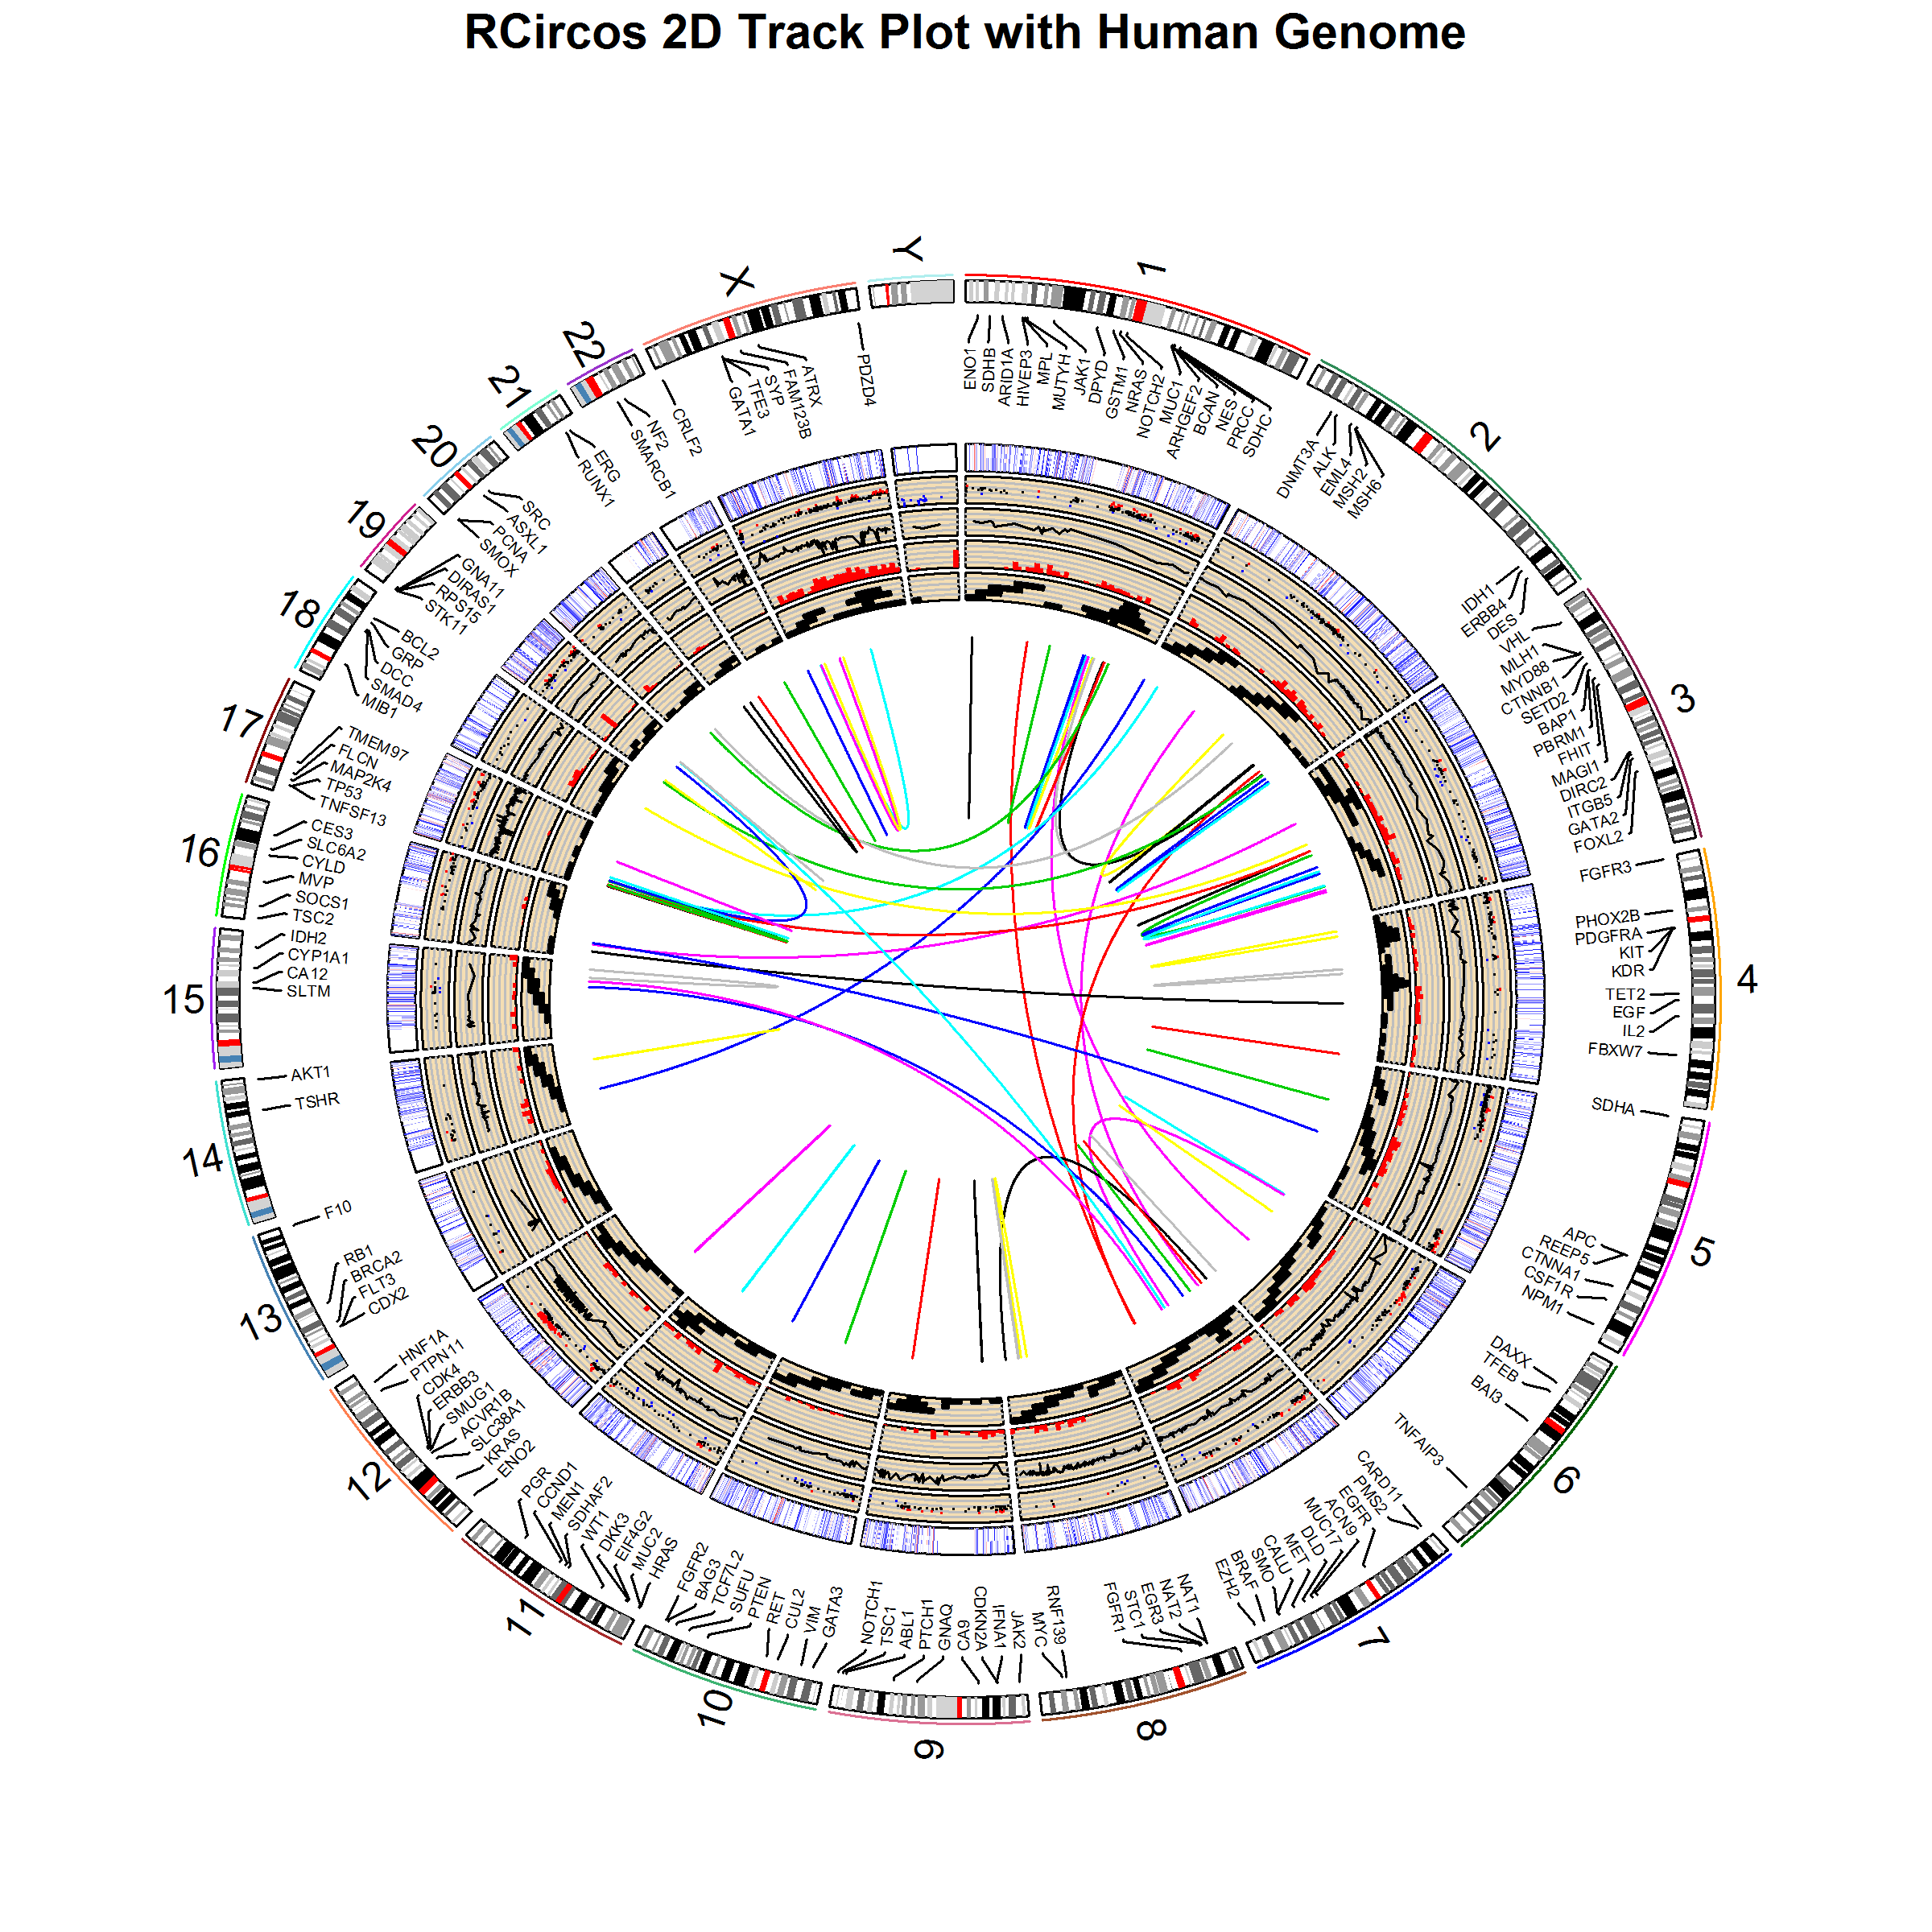
\includegraphics[width=1\textwidth]{RCircosDemoHuman.png}


\section{More Information}

Several demo samples are included in the package. Simply run following demos to see how the RCircos works for simple and complex Circos plot.

\begin{Schunk}
\begin{Sinput}
> library(RCircos);
> #	Same genome data and different plots
> #	************************************
> demo("RCircos.Demo.Human");
\end{Sinput}
\end{Schunk}

\begin{Schunk}
\begin{Sinput}
> #	Two diffent genomes and same plots
> #	************************************
> demo("RCircos.Demo.Mouse.And.Rat");
\end{Sinput}
\end{Schunk}

\section{sessionInfo}
\begin{Schunk}
\begin{Sinput}
> sessionInfo()
\end{Sinput}
\begin{Soutput}
R version 2.15.2 (2012-10-26)
Platform: x86_64-unknown-linux-gnu (64-bit)

locale:
[1] C

attached base packages:
[1] stats     graphics  grDevices utils     datasets  methods   base     

other attached packages:
[1] RCircos_1.0

loaded via a namespace (and not attached):
[1] tools_2.15.2
\end{Soutput}
\end{Schunk}

\begin{thebibliography}{1}
\bibitem{Krzywinski}  Krzywinski, Martin I and Schein, Jacqueline E and Birol, Inanc and Connors, Joseph and Gascoyne, Randy and Horsman, Doug and Jones, Steven J and Marra, Marco A.  Circos: An information aesthetic for comparative genomics. \textit{Genome Research}. 2009.
\end{thebibliography}

\end{document}
